%%%%%%%%%%%%%%%%%%%%%%%%%%%%%%%%%%%%%%%%%%%%%%%%%%%%%%%%%%%%%%%%%%%%
%%%%%%%%%%%%%%%%%%%%%%%%%%%%%%%%%%%%%%%%%%%%%%%%%%%%%%%%%%%%%%%%%%%%
%%                                                                %%
%% An example for writting your thesis using LaTeX                %%
%% Original version by Luis Costa,  changes by Perttu Puska       %%
%% Support for Swedish added 15092014                             %%
%%                                                                %%
%% This example consists of the files                             %%
%%         thesistemplate.tex (versio 2.01)                       %%
%%         opinnaytepohja.tex (versio 2.01) (for text in Finnish) %%
%%         aaltothesis.cls (versio 2.01)                          %%
%%         kuva1.eps                                              %%
%%         kuva2.eps                                              %%
%%         kuva1.pdf                                              %%
%%         kuva2.pdf                                              %%
%%                                                                %%
%%                                                                %%
%% Typeset either with                                            %%
%% latex:                                                         %%
%%             $ latex opinnaytepohja                             %%
%%             $ latex opinnaytepohja                             %%
%%                                                                %%
%%   Result is the file opinnayte.dvi, which                      %%
%%   is converted to ps format as follows:                        %%
%%                                                                %%
%%             $ dvips opinnaytepohja -o                          %%
%%                                                                %%
%%   and then to pdf as follows:                                  %%
%%                                                                %%
%%             $ ps2pdf opinnaytepohja.ps                         %%
%%                                                                %%
%% Or                                                             %%
%% pdflatex:                                                      %%
%%             $ pdflatex opinnaytepohja                          %%
%%             $ pdflatex opinnaytepohja                          %%
%%                                                                %%
%%   Result is the file opinnaytepohja.pdf                        %%
%%                                                                %%
%% Explanatory comments in this example begin with                %%
%% the characters %%, and changes that the user can make          %%
%% with the character %                                           %%
%%                                                                %%
%%%%%%%%%%%%%%%%%%%%%%%%%%%%%%%%%%%%%%%%%%%%%%%%%%%%%%%%%%%%%%%%%%%%
%%%%%%%%%%%%%%%%%%%%%%%%%%%%%%%%%%%%%%%%%%%%%%%%%%%%%%%%%%%%%%%%%%%%

%% Uncomment one of these:
%% the 1st when using pdflatex, which directly typesets your document in
%% pdf (use jpg or pdf figures), or
%% the 2nd when producing a ps file (use eps figures, don't use ps figures!).
\documentclass[english,12pt,a4paper,pdftex,sci,utf8]{aaltothesis}
%\documentclass[english,12pt,a4paper,dvips]{aaltothesis}

%% To the \documentclass above
%% specify your school: arts, biz, chem, elec, eng, sci
%% specify the character encoding scheme used by your editor: utf8, latin1

%% Use one of these if you write in Finnish (see the Finnish template):
%%
%\documentclass[finnish,12pt,a4paper,pdftex,elec,utf8]{aaltothesis}
%\documentclass[finnish,12pt,a4paper,dvips]{aaltothesis}

\usepackage{graphicx}
\usepackage{epstopdf}
\usepackage{fancyvrb}
\usepackage{tikz}
\usetikzlibrary{shapes,arrows,positioning,fit}

% Define block styles for tikz flow charts
\tikzstyle{decision} = [diamond, draw, fill=yellow!20, 
    text width=4.5em, text centered, node distance=3cm, inner sep=0pt]
\tikzstyle{block} = [rectangle, draw, fill=blue!20, 
    minimum width=5em, text centered, minimum height=4em]
\tikzstyle{thinblock} = [rectangle, draw, fill=black, 
    text width=0.01em, text centered, text height=1em]
\tikzstyle{line} = [draw, -latex']
\tikzstyle{cloud} = [draw, ellipse,fill=red!20, node distance=3cm,
    minimum height=2em]
\tikzstyle{every node}=[font=\small]
\tikzstyle{frame} = [line width=3pt, draw=cyan!80,dashed,inner sep=0.8em] %,minimum width=15cm,minimum height=6cm]
\tikzstyle{trapez} = [draw, trapezium, trapezium left angle=70, trapezium right angle=-70, minimum height=2em, fill=magenta!20]

%% Use this if you write hard core mathematics, these are usually needed
\usepackage{amsfonts,amssymb,amsbsy,amsmath}

%% Use the macros in this package to change how the hyperref package below 
%% typesets its hypertext -- hyperlink colour, font, etc. See the package
%% documentation. It also defines the \url macro, so use the package when 
%% not using the hyperref package.
%%
%\usepackage{url}

%% Use this if you want to get links and nice output. Works well with pdflatex.
\usepackage{hyperref}
\hypersetup{pdfpagemode=UseNone, pdfstartview=FitH,
  colorlinks=true,urlcolor=red,linkcolor=blue,citecolor=black,
  pdftitle={Default Title, Modify},pdfauthor={Your Name},
  pdfkeywords={Modify keywords}}


%% All that is printed on paper starts here
\begin{document}

%% Change the school field to specify your school if the automatically 
%% set name is wrong
% \university{aalto-yliopisto}
% \university{aalto University}
% \school{Sähkötekniikan korkeakoulu}
\school{School of Science}

%% Only for B.Sc. thesis: Choose your degree programme. 
\degreeprogram{Mathematics and Systems Analysis}
%%

%% ONLY FOR M.Sc. AND LICENTIATE THESIS: Specify your department,
%% professorship and professorship code. 
%%
%\department{Department of Radio Science and Technology}
%\professorship{Circuit theory}
%%

%% Valitse yksi näistä kolmesta
%%
%% Choose one of these:
\univdegree{BSc}
%\univdegree{MSc}
%\univdegree{Lic}

%% Your own name (should be self explanatory...)
\author{Pasi Pyrrö}

%% Your thesis title comes here and again before a possible abstract in
%% Finnish or Swedish . If the title is very long and latex does an
%% unsatisfactory job of breaking the lines, you will have to force a
%% linebreak with the \\ control character. 
%% Do not hyphenate titles.
%% 
\thesistitle{Lattice Codes and Sphere Decoding}

\place{Espoo}

%% For B.Sc. thesis use the date when you present your thesis. 
%% 
%% Kandidaatintyön päivämäärä on sen esityspäivämäärä! 
\date{14.8.2017}

%% B.Sc. or M.Sc. thesis supervisor 
%% Note the "\" after the comma. This forces the following space to be 
%% a normal interword space, not the space that starts a new sentence. 
%% This is done because the fullstop isn't the end of the sentence that
%% should be followed by a slightly longer space but is to be followed
%% by a regular space.
%%
\supervisor{Prof.\ Camilla Hollanti} %{Prof.\ Pirjo Professori}

%% B.Sc. or M.Sc. thesis advisors(s). You can give upto two advisors in
%% this template. Check with your supervisor how many official advisors
%% you can have.
%%
%\advisor{Prof.\ Pirjo Professori}
\advisor{Prof.\ Marcus Greferath}
\advisor{Dr.\ Oliver W. Gnilke}
%\advisor{M.Sc.\ Polli Pohjaaja}

%% Aalto logo: syntax:
%% \uselogo{aaltoRed|aaltoBlue|aaltoYellow|aaltoGray|aaltoGrayScale}{?|!|''}
%%
%% Logo language is set to be the same as the document language.
%% Logon kieli on sama kuin dokumentin kieli
%%
\uselogo{aaltoRed}{''}

%% Create the coverpage
%%
\makecoverpage


%% Note that when writting your master's thesis in English, place
%% the English abstract first followed by the possible Finnish abstract

%% English abstract.
%% All the information required in the abstract (your name, thesis title, etc.)
%% is used as specified above.
%% Specify keywords
%%
%% Kaikki tiivistelmässä tarvittava tieto (nimesi, työnnimi, jne.) käytetään
%% niin kuin se on yllä määritelty.
%% Avainsanat
%%
\keywords{sphere decoding, space--time lattice codes, wireless communications}
%% Abstract text
\begin{abstractpage}[english]
 \end{abstractpage}

%% Force a new page so that the possible English abstract starts on a new page
%%
%% Pakotetaan uusi sivu varmuuden vuoksi, jotta 
%% mahdollinen suomenkielinen ja englanninkielinen tiivistelmä
%% eivät tule vahingossakaan samalle sivulle

\newpage

%% Preface
%%
%% Esipuhe 
%\mysection{Preface}


%\vspace{5cm}
%Otaniemi, 16.1.2015

%\vspace{5mm}
%{\hfill Pasi Pyrrö \hspace{1cm}}

%% Force new page after preface
%\newpage


%% Table of contents.
\thesistableofcontents


%% Symbols and abbreviations
\mysection{Symbols and abbreviations}

\subsection*{Symbols}

\begin{tabular}{ll}
$\mathbb{Z}$  & Set of integers \\
$\mathbb{C}$  & Field of complex numbers \\
$\mathbf{x}$  & Vector \\
$\mathbf{X}$  & Matrix \\
\end{tabular}

\subsection*{Operators}

\begin{tabular}{ll}
$\| \cdot \| $     & Euclidean norm \\
$\left\lceil\cdot\right\rfloor$ & Round to nearest integer \\
det$(\mathbf{X})$  & Determinant of matrix $\mathbf{X}$
\end{tabular}

\subsection*{Abbreviations}

\begin{tabular}{ll}
SNR & Signal to noise ratio \\
CVP & Closest vector problem \\
MIMO & Multiple input multiple output \\
PAM & Pulse amplitude modulation \\
i.i.d. & independent and identically distributed \\
BLER & Block error rate \\
\end{tabular}


%% Tweaks the page numbering to meet the requirement of the thesis format:
%% Begin the pagenumbering in Arabian numerals (and leave the first page
%% of the text body empty, see \thispagestyle{empty} below).
%% Additionally, force the actual text to begin on a new page with the 
%% \clearpage command.
%% \clearpage is similar to \newpage, but it also flushes the floats (figures
%% and tables).
%% There is no need to change these
%%
\cleardoublepage
\storeinipagenumber
\pagenumbering{arabic}
\setcounter{page}{1}


%% Text body begins. Note that since the text body
%% is mostly in Finnish the majority of comments are
%% also in Finnish after this point. There is no point in explaining
%% Finnish-language specific thesis conventions in English. Someday 
%% this text will possibly be translated to English.
%%
\section{Introduction}
%% Leave first page empty
Wireless communication has been a crucial part of modern information technology for a couple of decades now. It is facing a lot of practical everyday problems which motivate the ongoing extensive research on the field. One of these problems is the noise and fading that occurs on wireless channels due to obstacles and radiation from the surroundings. To avoid data loss during transmission via wireless link one has to encode the data to be sent in such a robust way that it can still be recovered at the receiving end even in the presence of noise and fading of reasonable scale. 
\par One way to tackle this problem, and the method this thesis focuses on, is the use of space--time lattice codes and sphere decoding. From a mathematical point of view the process of decoding can then be viewed as a problem of finding the closest lattice point to a given input vector, that is, the possibly noisy vector containing the data we receive from the wireless channel. This problem in its general form is known to be NP-hard, but for communications applications, where the dimensionality and the shape of the lattice are kept reasonable, there exist algorithms, like the sphere decoder, that offer polynomial expected complexity with respect to the size of the codeword constellation \cite{mia}.


%% In a thesis, every section starts a new page, hence \clearpage
\clearpage

\section{Lattices in communications technology}

Before we go into communications applications of lattices such as lattice codes, let us start off with the definition of a lattice. Let $n$ and $m$ be positive integers such that $n \leq m$ and $\mathbf{b}_1, ... , \mathbf{b}_n \in \mathbb{R}^m$ be linearly independent vectors. A discrete Abelian subgroup $\Lambda$ of $\mathbb{R}^m$ is called a \emph{lattice} of dimension $n$ if it is defined as

\begin{equation}
\Lambda = \sum_{i=1}^{n} \mathbb{Z}\mathbf{b}_i = \{a_1\mathbf{b}_1 + \ldots + a_n\mathbf{b}_n \mid a_i \in \mathbb{Z}, 1 \leq i \leq n\}\label{eq:lattice}
\end{equation}

\noindent where the set of vectors $\mathbf{b}_1, \ldots, \mathbf{b}_n \in \mathbb{R}^m$ is called the basis of the lattice $\Lambda$. All points of the lattice can be obtained as a linear combination of the basis vectors $\mathbf{b}_i$ and integer coefficients $\mathbf{a}_i$ as stated in \eqref{eq:lattice}. The number of basis vectors $n$ is also called the rank of the lattice and if $n = m$ the lattice is said to have full rank. The points of the lattice $\Lambda$ form a group under addition which means that if $\mathbf{x} \in \Lambda$ then $-\mathbf{x} \in \Lambda$ and if $\mathbf{x}, \mathbf{y} \in \Lambda$ then $\mathbf{x} \pm \mathbf{y} \in \Lambda$. \cite{cassels}
\par There is also a matrix representation for the same lattice
\begin{equation}
\Lambda = \{\mathbf{B}a \mid a \in {\mathbb Z}^n\} \label{eq:matrix}
\end{equation}
where $\mathbf{B} = [\mathbf{b}_1, ... , \mathbf{b}_n]$ is an $m \times n$ matrix called the generator matrix of the lattice $\Lambda$ and $\mathbf{a}$ is an $n$-dimensional integer column vector. Note that $\mathbf{B}$ is not uniquely determined by the lattice as in fact there exists infinitely many bases for the same lattice \cite{cassels}. Also the origin is part of every lattice regardless of the choice of $\mathbf{B}$. If $\mathbf{B}$ is a basis for lattice $\Lambda$ then $\mathbf{B}'$ is also a basis for the same lattice if the following holds
\begin{align}
\mathbf{B}' &= \mathbf{W}\mathbf{B}, \\
\text{det}(\mathbf{W}) &= \pm 1
\label{eq:basis_change}
\end{align}
where $\mathbf{W}$ is an $m \times m$ matrix with integer entries \cite{agrell}. Some bases are however better in some sense than others, especially in communications applications, as one could imagine. Usually reasonable orthogonality and relatively small norm for the basis vectors are desired \cite{agrell}. A better basis can be obtained via a process called basis reduction, which is illustrated in figure \ref{fig:bases}. Clearly basis vectors $\mathbf{u}_i$ obtained from the basis reduction are more pleasant to work with than the original vectors $\mathbf{v}_i$ although they both span the same lattice.

\begin{figure}[ht]
  \centering
  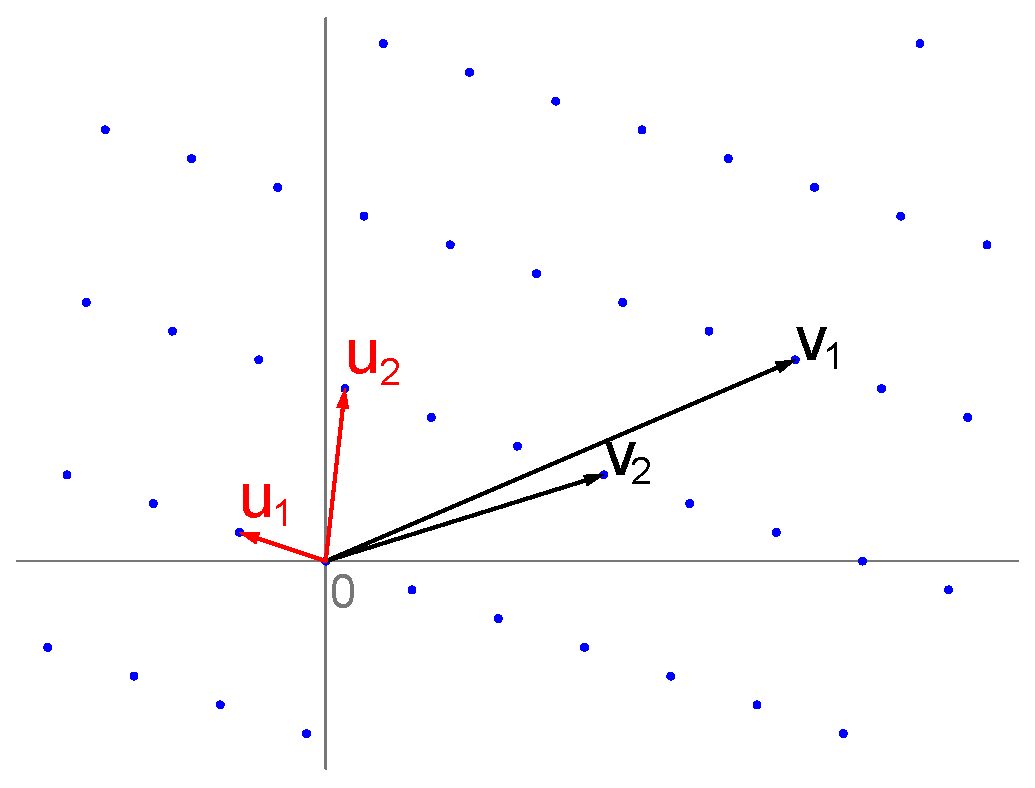
\includegraphics[width=0.8\linewidth]{Lattice-reduction}
  \caption{Two different bases for the same two dimensional lattice.}
  \label{fig:bases}
\end{figure}

\par What we considered earlier were lattices spanned over real $m$-dimensional space $\mathbb{R}^m$ but in similar sense we can consider a lattice consisting of complex valued vectors from $\mathbb{C}^m$. The principles of such complex lattice are almost the same, however, now elements of $\mathbf{B}$ and $\mathbf{a}$ take values from $\mathbb{C}$. Note that a complex lattice has an equivalent real representation which has double the rank of the corresponding complex lattice. Consider a lattice $\Lambda \subset \mathbb{C}^m$ with a generator matrix $\mathbf{B} = [\mathbf{z}_1, ... , \mathbf{z}_n]$. Now we can always express it with a real valued lattice $\Lambda_{\text{real}} \subset \mathbb{R}^{2m}$ and the corresponding $2m \times n$ generator matrix is given by

\begin{equation}
\mathbf{B}_{\text{real}} =
\begin{bmatrix} 
\text{Re}(z_{11}) & \dots  & \text{Re}(z_{1n}) \\
\text{Im}(z_{11}) & \dots  & \text{Im}(z_{1n}) \\
\vdots            & \ddots & \vdots            \\
\text{Re}(z_{m1}) & \dots  & \text{Re}(z_{mn}) \\
\text{Im}(z_{m1}) & \dots  & \text{Im}(z_{mn}) \\
\end{bmatrix}.
\label{eq:complex}
\end{equation}
In other words we convert each column of $\mathbf{B}$ to real vector by separating each of their complex elements into two adjacent real elements, that is the real and imaginary parts of the original complex element. This process doubles the amount of rows in $\mathbf{B}_{\text{real}}$ but both representations ultimately describe the same lattice. \cite{conway}

\subsection{Closest vector problem}

The most relevant mathematical problem related to sphere decoding, a communications application of interest in this paper, is the closest vector problem (CVP). Let $J$ be a general vector space. Given a lattice $\Lambda \subset J$ and an input point $\mathbf{y} \in J$ the problem is to find a lattice point $\hat{\mathbf{x}} \in \Lambda$ that is closest to $\mathbf{y}$. More precisely $\hat{\mathbf{x}} \in \Lambda$ has to meet the following condition

\begin{equation}
\|\mathbf{y}-\hat{\mathbf{x}}\| \leq \|\mathbf{y}-\mathbf{x}\|, \ \ \ \forall \mathbf{x} \in \Lambda.
\label{eq:cvp}
\end{equation}

\noindent In this thesis we mostly consider $J=\mathbb{C}^n$. 
\par For a fixed point $\mathbf{x}' \in \Lambda$ the set of vectors $\mathbf{y}_i \in J$ that satisfy the inequality \eqref{eq:cvp} is called the Voronoi region $\mathcal{V}_{\mathbf{x}'} \subset J$ (see figure \ref{fig:voronoi}) of lattice point $\mathbf{x}'$ \cite{zamir}. This means that if $\mathbf{y} \in \mathcal{V}_{\mathbf{x}'}$ then the solution to CVP is $\mathbf{x}'$. An example of lattice's Voronoi cells is illustrated in figure \ref{fig:voronoi}. If $\mathbf{y} \in \partial\mathcal{V}_{\mathbf{x}'}$ the solution to CVP is a random choice between points whose Voronoi region contains that boundary. The volume of the $\mathcal{V}_{\mathbf{x}'}$
%, also known as the lattice constant as it is independent of the choice of basis, 
is given by det$(\Lambda) = $ $\sqrt{\text{det}(\mathbf{B}^T\mathbf{B}})$, where $\mathbf{B}$ is the generator matrix of $\Lambda$. 

\begin{figure}[ht]
% source: http://www.gregegan.net/APPLETS/12/deBruijnNotes.html
  \centering
  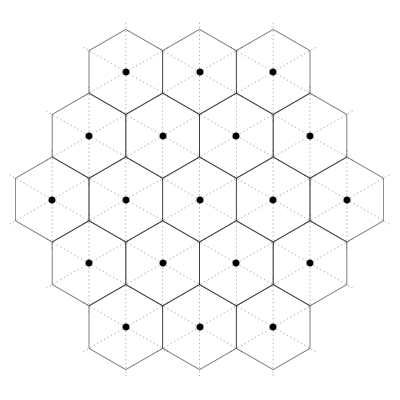
\includegraphics[width=0.5\linewidth]{voronoi_cells}
  \caption{The Voronoi cells of the two dimensional hexagonal lattice $\mathsf{A}_2$.}
  \label{fig:voronoi}
\end{figure}

CVP is trivial for orthogonal lattices as one could just round every coordinate of $\mathbf{y}$ to nearest integer an get the correct answer, but CVP has been shown to be NP-hard as the function of the lattice rank in general case when we consider skewed lattices and thus all known algorithms for CVP have exponential worst case complexity \cite{agrell}. Non-trivial lattices appear in most communications applications, for example when using maximum likelihood decoding for lattice codes sent via channel that induces fading. Such decoding process can be thought as a CVP. %and it's later explained in further detail.

\subsection{Space--time lattice codes}

Space--time lattice codes are a robust way of encoding the data on a  wireless channel that uses multiple transmit and receiver antennas, i.e. a MIMO-system. Wireless channels are usually very error prone due to interference and fading caused by the surrounding electrical devices, obstacles and environment. This method helps to improve the reliability of the data transmission on such channel, meaning we get decoding errors less likely. Codebook from a certain space--time lattice code constellation can be represented as a set of matrices, which is defined as

\begin{equation}
\mathcal{L} = \Bigg\{\sum_{i=1}^k a_i\mathbf{X}_i \ \Big| \ \mathbf{X}_i \in \mathcal{M}_{m \times l}(\mathbb{C}), \ a_i \in S \subset \mathbb{Z} \Bigg\}.
\label{eq:codeword}
\end{equation}
The $\mathbf{X}_i, i = 1,...,k$ denote the constant basis matrices of the lattice code and the coefficients $a_i, i = 1,...,k$ are integers from a finite signal set $S$ which represent the data we want to send. We call $\mathcal{L}$ our codebook as it contains all possible codewords for a certain finite signal set. In this thesis we consider the pulse amplitude modulation ($q$-PAM) signal set of size $q$. It is defined as

\begin{equation}
S = \{a = 2u-q+1\mid u \in \mathbb{Z}_q\}
\label{eq:pam}
\end{equation}
with $\mathbb{Z}_q = \{0,1,...,q-1\}$. So for example 4-PAM gives $S = \{-3, -1,1,3\}$ i.e. all the odd integers which absolute value is smaller than 4. The size of the signal set is usually chosen to be some power of two, i.e. $q = 2^b$. This way $b$ information bits are mapped to each codeword we send. \cite{mia} 
%Note that the origin i.e. the zero vector is never part of the $q$-PAM codebook $\mathcal{L}$ as it maps to origin in every lattice we choose for our lattice code.

\begin{figure}[ht]
  \centering
  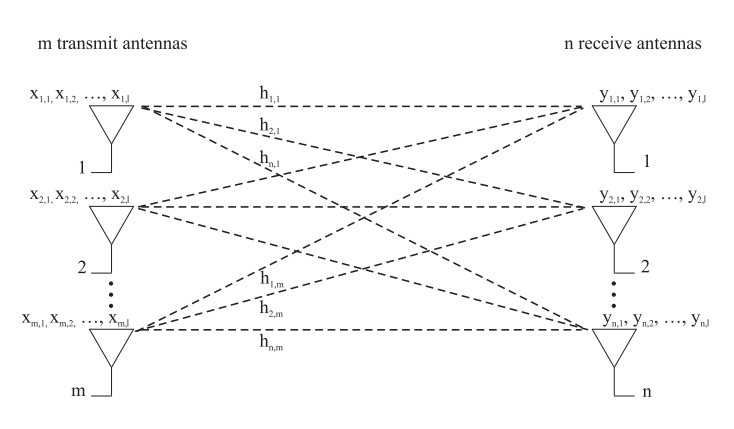
\includegraphics[width=\linewidth]{mimo}
  \caption{The MIMO-channel model with quasi-static Rayleigh fading \cite{mia}.}
  \label{fig:mimo}
\end{figure}

\par Consider a multiple antenna system as in figure \ref{fig:mimo} of $m$ transmit and $n$ receive antennas. We choose an $m\times l$ complex matrix $\mathbf{X} \in \mathcal{L}$ constructed from \eqref{eq:codeword} as the codeword which we send through this wireless channel, where $l$ denotes the number of channel uses (time slots) required to send the codeword. In this thesis we consider quasi-static channel model i.e. path gains $h_{i,j}$ in figure \ref{fig:mimo} are assumed to stay constant during the sending of single codeword i.e. during $l$ channel uses and then change. 
%To simulate noise we must add a matrix whose entries are identically distributed complex Gaussian random variables to the codeword we receive. 
\par The simulated received noisy $m\times l$ codeword matrix can be obtained like this

\begin{equation}
\mathbf{Y} = \mathbf{HX} + \mathbf{N}
\label{eq:system}
\end{equation}

where $\mathbf{H}$ is $n \times m$ channel matrix that simulates the path gains in figure \ref{fig:mimo} and $\mathbf{N}$ is a $n\times l$ noise matrix. $\mathbf{H}$ and $\mathbf{N}$ is generated from independent and identically distributed  (i.i.d.) complex Gaussian random entries with zero mean for each simulation round. Their distributions use different variance though. 
\par The component $y_{i,j}$ of the received matrix corresponds to the $j$-th signal received by antenna $i$, which is a superposition of faded versions of all $m$ transmitted signals with additive noise, i.e. it can be obtained like
\begin{equation}
y_{i,j} = h_{i,1}x_{1,j}+h_{i,2}x_{2,j}+...+h_{i,m}x_{m,j}+n_{i,j}   
\label{eq:component}
\end{equation}
for all $1 \leq i \leq n, \ 1 \leq j \leq m$. The $n_{i,j}$ is the corresponding noise matrix component.
\par The problem of decoding is now: Given $\mathbf{Y}$, which $\mathbf{X} \in \mathcal{L}$ was sent? According to maximum likehood principle this can be viewed as CVP \cite{mia} and is discussed in the next chapter in further detail.

\clearpage

\section{Sphere decoder}

In this chapter we will discuss an efficient decoding algorithm for space--time block codes known as the sphere decoder. The name \emph{sphere decoder} actually comes from Pohst's idea of conducting the search within a finite hypersphere in 1981 \cite{agrell}. This thesis is particularly interested in the Schnorr-Euchner implementation of the algorithm, which is based on Pohst strategy and the Babai nearest plane algorithm \cite{agrell}. 
\par The problem of decoding the correct codeword from the set of all possible codewords from the received noisy codeword can be reduced to CVP discussed earlier \cite{mia}. But exhaustive search over all points (codewords) in the finite lattice of interest (codebook) is just not feasible solution as the number of possible codewords grows exponentially with the rank of the lattice code $k$ in equation \eqref{eq:codeword} and the size of the signaling set $q$ in equation \eqref{eq:pam}. 
\par Luckily the sphere decoder algorithm exists, which instead of searching through all lattice points within the finite signal set boundaries only considers lattice points within a hypersphere around the received vector of certain radius like in figure \ref{fig:sphere}. This significantly reduces the complexity of the search algorithm. 

\begin{figure}[ht]
  \centering
  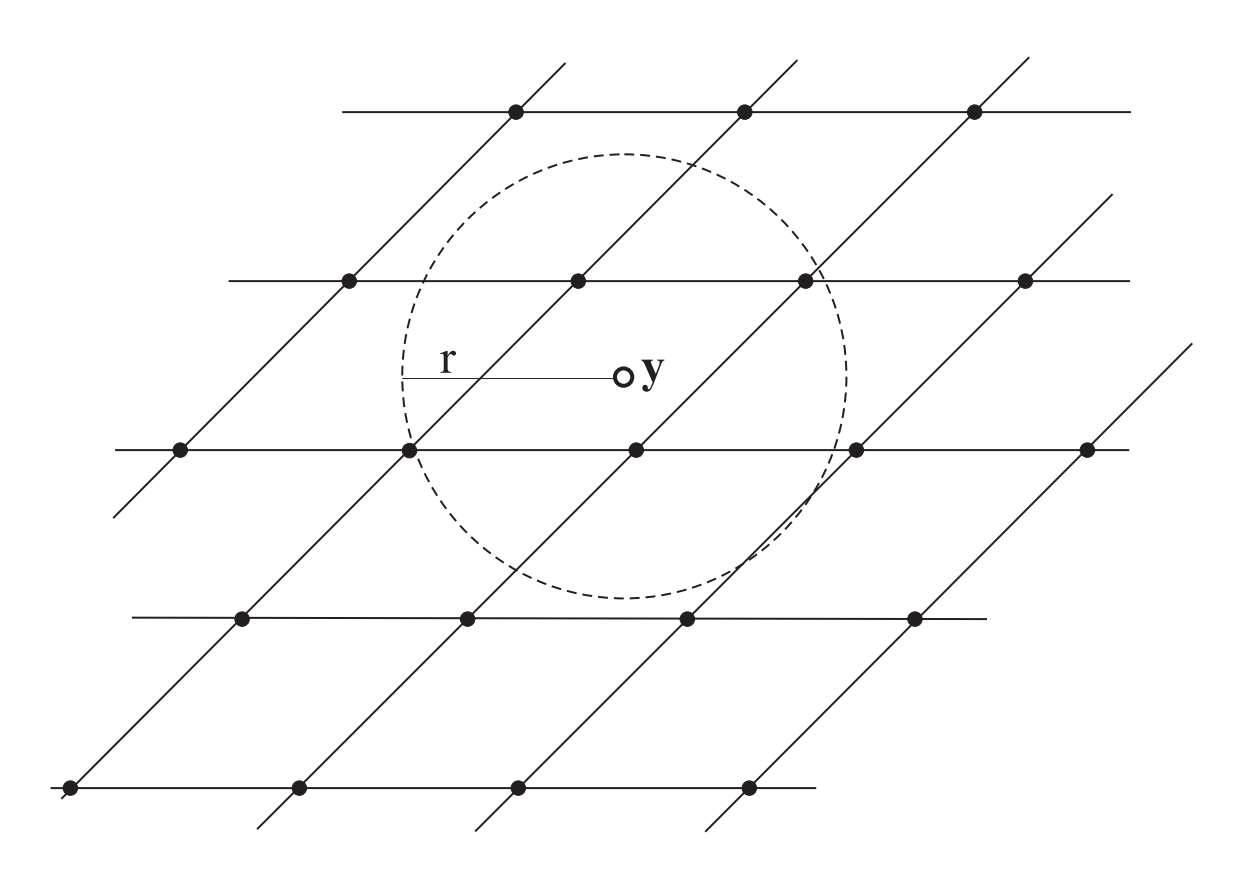
\includegraphics[width=0.8\linewidth]{sphere_decoder}
  \caption{The CVP with sphere decoding in two dimensional lattice. The search complexity can be reduced by giving an upper bound for the closest point distance \cite{mia}.}
  \label{fig:sphere}
\end{figure}

Although one can do even better than that: everytime the algorithm finds a lattice point within the hypersphere and one is interested in finding the closest one, one can obviously shrink down the search radius. It is now sufficient to only consider lattice points that are either as far away as the point the algorithm just found, or lattice points that are closer, thus the search radius can be set to equal the distance to that point.
\par There is however still the problem of choosing the initial radius for the sphere decoder. In simulations one can always \emph{cheat} and set the radius roughly equal the power of the noise we apply to the system. In real life applications however, where we cannot predict the power of the noise in the channel, this is not trivial task for some implementations of sphere decocer. Luckily the Schnorr-Euchner strategy, which this paper is interested in, uses Babai nearest plane algorithm as a part of its implementation, which guarantees the algorithm always finds a nearby point without any initial radius at all. Once it finds a lattice point that is reasonably near the codeword that was received, the algorithm can use its distance as the upper bound for the sphere decoder and only consider lattice points that are within that radius from that point on.

%\par One question remains though, so how do we choose the radius? If it's too small, no lattice points lie within the sphere or if it's too large, the complexity will increase and slow down the algorithm. In ideal case the answer to that question is, with our Schnorr-Euchner implementation of the algorithm, we can simply set it to infinity. It uses by definition the Babai nearest plane algorithm, which requires no upper bound for the distance to the closest point to find a nearby point which we can use to dynamically update the upper bound of the search algorithm to the distance to that point.  Clearly the closest point is either that point we just found, also known as the Babai point, or another one within that radius. 
\par However since in practise we consider finite subsets of the lattice, there is a possibility that the Babai point lies outside of the codebook region, which causes the algorithm to loop infinitely \cite{agrell}. To avoid this the Algorithm 1 and 2 introduced in this paper, which are both modifications of the Schnorr-Euchner strategy, consider only lattice points that have values taken from the chosen finite signal set as their components. %Some modules for estimating the radius for a codebook of given size have been also implemented in the program itself. 
The real benefit of the integrated Babai algorithm in Schnorr-Euchner strategy comes from the increased probability of finding the closest lattice point early at the cost of slightly increased computational complexity compared to Pohst strategy \cite{agrell}. 

\subsection{Recursive sublattice decomposition}

For understanding how the sphere decoder works let us introduce the concept of sublattice decomposition from $n$-dimensional lattice to a stack of $(n-1)$-dimensional sublattices. As one could guess this can also be done recursively and ultimately we end up with 0-dimensional lattices also known as the lattice points. The motivation to this recursive representation of a lattice is that one only needs to consider intervals of sublattice layer indices when doing the distance comparison in each dimension from $n$ to $0$.
\par Let us consider a $m \times n$ lattice generator matrix $\mathbf{G}$ for a lattice $\Lambda$ and write it like
 
\begin{equation}
\mathbf{G} = \big[\mathbf{G}' \ \ \mathbf{v}_n \big]
\label{eq:gen}
\end{equation}
where $\mathbf{G}'$ is a $m \times (n-1)$ matrix and the last column vector can be written as $\mathbf{v}_n = \mathbf{v}_{\parallel} + \mathbf{v}_{\bot}$, with $\mathbf{v}_{\parallel}$ in the column space of $\mathbf{G}'$ and $\mathbf{v}_{\bot}$ in the null space of $\mathbf{G}'$. With this notation we can decompose any $n$-dimensional lattice as follows

\begin{equation}
\Lambda(\mathbf{G}) = \bigcup_{u_n=-\infty}^{+\infty} \big\{\mathbf{c}+u_n\mathbf{v}_{\parallel}+u_n\mathbf{v}_{\bot} \mid \mathbf{c} \in \Lambda(\mathbf{G}'), \ u_n \in \mathbb{Z} \big\}.
\label{eq:decom}
\end{equation}

\noindent Equation \eqref{eq:decom} basically describes a stack of $(n-1)$-dimensional translated sublattices, where $u_n$ is the index of each sublattice of an $n$-dimensional lattice $\Lambda$. The hyperplanes over which the sublattices are spanned are called \textit{layers}. For example you can think of the horizontal lines in figure \ref{fig:sphere} as one dimensional layers and the discrete points in them as sublattices of the whole two dimensional lattice.
\par To better understand the given expression in equation \eqref{eq:decom} let's consider the sublattice in the base layer $u_n = 0$, which is just all the points in the sublattice generated by $\mathbf{G}'$. Similarly we can get all other sublattices from this base sublattice by offsetting all the points in it by linear combination $u_n\mathbf{v}_{\parallel}+u_n\mathbf{v}_{\bot}$, where $\mathbf{v}_{\parallel}$ denotes a translation of all points in that same hyperplane and $\|\mathbf{v}_{\bot}\|$ is the orthogonal distance between two adjacent layers in the $n$-th dimension. By taking the union of all these sublattices we get the whole $n$-dimensional lattice. In figure \ref{fig:sphere} for example you can think of the middle horizontal line as the base layer.
\par If $\mathbf{G}$ is an upper triangular matrix, we can easily express $\mathbf{v}_{\bot}$ as $\mathbf{v}_{\bot} = (0, 0, ..., v_{nn})^T$ and thus we can write simply $\|\mathbf{v}_{\bot}\| = |v_{nn}|$. In fact any generator matrix $\mathbf{G}$ can be rotated to upper triangular form \cite{agrell} with $v_{nn} > 0$ so we can simply denote the distance between $(k-1)$-dimensional layers with $v_{kk}$ later on.
\par With the concept of recursive sublattice decomposition, CVP in $n$-dimensional lattice $\Lambda(\mathbf{G})$ can be done recursively with a finite number of ($n-1$)-dimensional search operations. If $\mathbf{x} \in \mathbb{R}^m$ is a vector to decode in the lattice $\Lambda(\mathbf{G})$, which is decomposed as in \eqref{eq:decom}, the orthogonal distance $y_n$ from $\mathbf{x}$ to the $(n-1)$-dimensional layer with index $u_n$ is given by the formula
\begin{equation}
y_n = |u_n-\hat{u}_n| \cdot \|\mathbf{v}_{\bot}\|
\label{eq:dist}
\end{equation}
where
\begin{equation}
\hat{u}_n = \frac{\mathbf{xv}_{\bot}^t}{\|\mathbf{v}_{\bot}\|^2}
\label{eq:uhat}
\end{equation}
i.e. $\hat{u}_n$ is a scalar projection of $\mathbf{x}$ onto $\mathbf{v}_{\bot}$. %the $(n-1)$-dimensional layer (hyperplane). 
Inserting this scalar projection i.e. the magnitude of $\mathbf{x}$ vector's orthogonal component %wrt. to the layers in dimension $n$ 
into the equation \eqref{eq:dist} pretty obviously yields the orthogonal distance of $\mathbf{x}$ to the layer with index $u_n$. This is illustrated in figure \ref{fig:sublattice}.

\begin{figure}[ht]
\centering
\begin{tikzpicture}[auto]
	% Place nodes
	%\node [thinblock] (start) {a};
	%\node [thinblock, right of=start, node distance=1em] (ni) {b};
	
	\draw (5.5,0.5) -- coordinate (x axis mid) (6,0.5);
	\draw (5.5,0.4) -- (5.5,0.6) node[anchor=south] {};
	\draw (5.75,0.5) -- (5.75,0.5) node[anchor=south] {$y_n$};
	\draw (6,0.4) -- (6,0.6) node[anchor=south] {};
	
	\draw (0,0.5) -- coordinate (x axis mid) (2,0.5);
	\draw (0,0.4) -- (0,0.6) node[anchor=south] {};
	\draw (1,0.5) -- (1,0.5) node[anchor=south] {$\|\mathbf{v}_{\bot}\|$};
	\draw (2,0.4) -- (2,0.6) node[anchor=south] {};
	
	\draw (-1,0) -- coordinate (x axis mid) (11,0);
	\draw (0,5pt) -- (0,-5pt) node[anchor=north] {-2};
	\draw (2,5pt) -- (2,-5pt) node[anchor=north] {-1};
	\draw (4,5pt) -- (4,-5pt) node[anchor=north] {0};
	\draw (5.5,2pt) -- (5.5,-2pt) node[anchor=north] {$\mathbf{x}$};
	\draw (6,5pt) -- (6,-5pt) node[anchor=north, align=center] {1 \\ $\left\lceil\hat{u}_n\right\rfloor$};
	\draw (8,5pt) -- (8,-5pt) node[anchor=north] {2};
	\draw (10,5pt) -- (10,-5pt) node[anchor=north] {3};
	
	\node[below=0.2cm] at (10.8,-0.3) {$u_n$};
 
\end{tikzpicture}
\caption{A stack of parallel layers of an $n$-dimensional lattice. $u_n$ denotes the layer index.}
\label{fig:sublattice}
\end{figure} 


\subsection{Schnorr-Euchner lattice search algorithm}
Now regarding CVP it is sufficient to consider these orthogonal distances in equation \eqref{eq:dist} and we can thus write the CVP as
\begin{equation}
\mathbf{\hat{x}} = 
\underset{\mathbf{x}\,\in\,\Lambda(\mathbf{G})}{\operatorname{argmin}} 
\sum_{n = 0}^{m} y_n
\label{eq:cvp}
\end{equation}
where $\mathbf{\hat{x}}$ is the lattice point closest to $\mathbf{x}$. This can be thought as traversing a search tree of depth $m$ from root node to the leaf node at lowest level with smallest sum of vertex weights. In the figure \ref{fig:tree} a search tree for 4-dimensional CVP is illustrated. The tree is not full as not all subtrees need to be considered in smart implementations of the lattice search algorithm as the search can be stopped early. Note that only paths from root to level 4 nodes are considered feasible solutions to CVP as the solution vector $\mathbf{\hat{x}}$ has to have 4 components.
\begin{figure}[ht] 
  \centering
  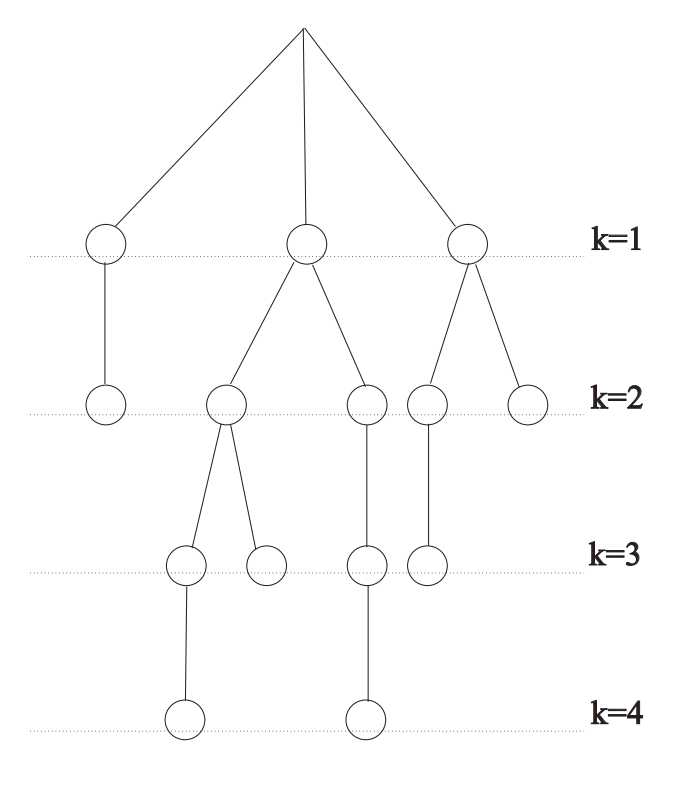
\includegraphics[width=0.5\linewidth]{search-tree}
  \caption{Traversal of a lattice search algorithm in a four dimensional lattice \cite{mia}.}
  \label{fig:tree}
\end{figure}
The node values on each level $k$ of the search tree represent candidate value for the $(m-k+1)$-th component of the solution vector selected from some finite signal set. Here $m = 4$.
\par So how does one select the layer, which is closest to $\mathbf{\hat{x}}$ in each dimension $n$? As the layer indices $u_n$ take values from $\mathbb{Z}$, clearly selecting $u_n = \left\lceil\hat{u}_n\right\rfloor$ in equation \eqref{eq:dist} gives you the smallest $y_n$ in that dimension. 
%The operation $\left\lceil\cdot\right\rfloor$ denotes rounding to the nearest integer. 
Considering only this option in each dimension yields the Babai nearest plane algorithm, which reduces the search problem to a $(m-1)$-dimensional one. It is a quick way to find a nearby lattice point, but it is not necessarily the closest one \cite{agrell}. The point found by this algorithm is called the Babai point.
\par To ensure one indeed finds the closest lattice point, which in decoding applications like the sphere decoder is crucial, one needs to be a bit more throughout than this. Indeed Schnorr-Euchnerr sphere decoder does not stop here but instead climbs up the search tree and enumerates through all feasible points that are closer than the first point found also known as the \emph{Babai point}. This what the sphere decoder using Pohst strategy would also do. What's different in Schnorr-Euchner strategy from Pohst apart from not requiring initial radius thanks to the Babai nearest plane algorithm is the way of enumerating sublattice indices in equation \eqref{eq:dist}. While Pohst method would just go through the layers in ascending order within the distance upper bound (sphere radius), Schnorr-Euchnerr starts from the midpoint i.e. $u_n = \left\lceil\hat{u}_n\right\rfloor$ and zigzags around it until it hits the upper bound (see figure \ref{fig:sublattice}). In other words the Schnorr-Euchner enumeration goes through the layers in ascending order of the orthogonal distances $y_n$. The benefit of doing this is quite obvious: if one finds a layer $u_n$ that is outside the current sphere radius one can stop the search in that sublattice early, as clearly there are no longer points within radius in that sublattice, thanks to the ascending distance ordering. This significantly reduces the search tree complexity depicted in figure \ref{fig:tree} and thus makes the algorithm more efficient \cite{mia}\cite{agrell}.

\subsection{Sphere decoder implementation}
The sphere decoder algorithm used by the program is a modification of the Schnorr-Euchner strategy described earlier which also accounts for finite signal set boundaries with some optimizations. It is based on the algorithms introduced in \cite{mia} and \cite{ranto}, but there are a couple of key differences. The new implementation natively handles $q$-PAM signal sets defined in equation \eqref{eq:pam}, so the signal set does not need to be mapped to interval $[0,q-1]$ first like in previous algorithms, which was confusing when comparing the input and output vectors. The program also uses the dedicated and efficient linear algebra library called \emph{Armadillo} \cite{arma}. The library also has intuitive syntax, which makes the code rather easy to read for those who wish to understand every detail of it. While the original algorithm in \cite{ranto} also handled spherically shaped codebooks, this program introduces two separate algorithms: one for parallelotope and one for spherically shaped codebooks. Pseudocodes for both algorithms are given in this paper. This division saves a lot of unnecessary comparisons when using the program with a normal pallelotope shaped codebook, which not surpricingly requires a much simpler algorithm. 
\par The way the algorithms in the program are structured, provides a lot of modularity. This gives the experienced user with programming background an option to program his or her own custom simulations using this application programming interface within the main program source file.
\par The sphere decoder consist of two parts: \emph{input preprocessing} and \emph{decoding} as can be seen in figure \ref{fig:sphdec}.

%The program is written in C++11 and uses a linear algebra library called Armadillo \cite{arma} for most matrix and vector operations. It is primarily designed for Unix operating systems but should be portable to other systems as well with slight modifications although not all features are quaranteed to work optimally.
\begin{figure}[ht]
\centering
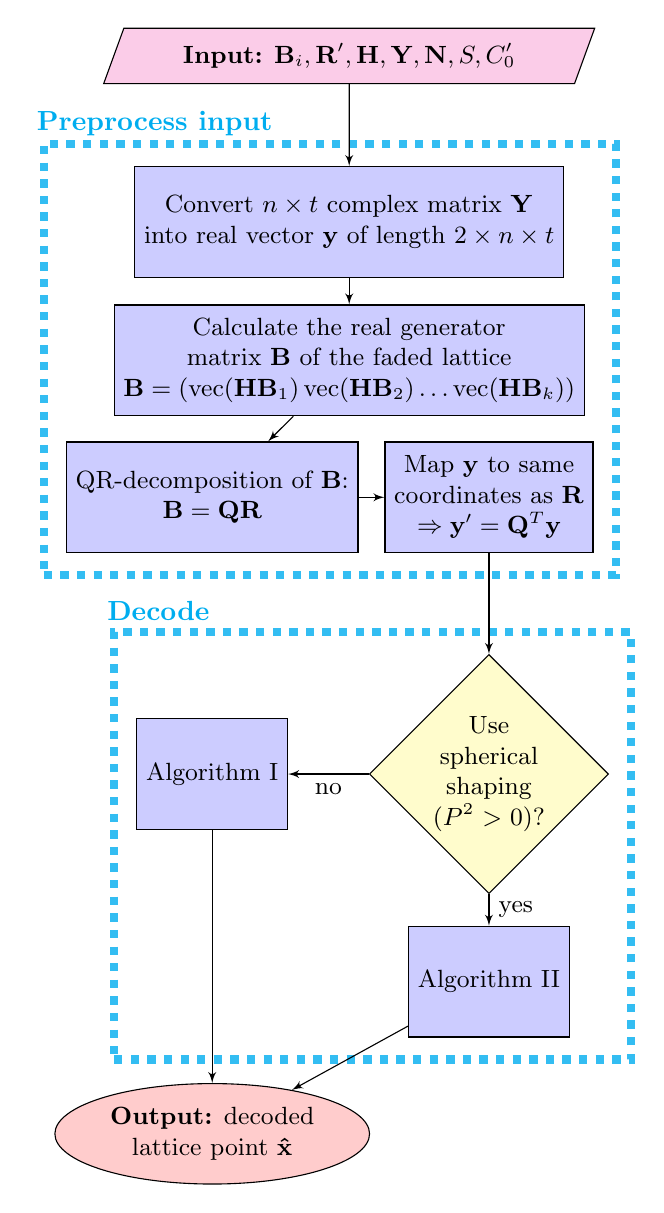
\begin{tikzpicture}[node distance = 5em, auto]
	% Place nodes
	\node [trapez, align=center] (input) {\textbf{Input:} $\mathbf{B}_i, \textbf{R}', \textbf{H}, \textbf{Y}, \textbf{N}, S, C'_0$};
	\node [block, align=center, below of=input, node distance=6em] (start) {Convert $n\times t$ complex matrix $\mathbf{Y}$\\ into real vector $\textbf{y}$ of length $2\times n\times t$};
	\node [block, align=center, below of=start] (gen) {Calculate the real generator \\ matrix $\textbf{B}$ of the faded lattice \\ $\mathbf{B} = \left(\text{vec}(\textbf{H}\textbf{B}_1) \,\text{vec}(\textbf{H}\textbf{B}_2) \ldots \text{vec}(\textbf{H}\textbf{B}_k)\right)$};
	\node [block, align=center, below left of=gen, node distance=7em] (qr) {QR-decomposition of $\mathbf{B}$: \\ $\textbf{B} = \textbf{QR}$}; 
	\node [block, align=center, right of=qr, node distance=10em] (mapy) {Map $\mathbf{y}$ to same \\ coordinates as $\textbf{R}$\\ $\Rightarrow \textbf{y}' = \mathbf{Q}^T \textbf{y}$};
	
	%frame 1
	\node [frame,fit=(start)(qr)(gen)(mapy)] (cyan) {};
	\node [anchor=south west, font=\color{cyan}\bf, xshift=-0.45em, yshift=-0.2em] at (cyan.north west){Preprocess input};
	
	\node [decision, below of=mapy, node distance=10em] (choose) {Use spherical shaping ($P^2 > 0$)?};
	\node [block, align=center, below of=choose, node distance=7.5em] (alg_ii) {Algorithm II}; 
	\node [block, align=center, left of=choose, node distance=10em] (alg_i) {Algorithm I}; 
	\node [cloud, align=center, below of=alg_i, node distance=13em] (output) {\textbf{Output:} decoded \\ lattice point $\mathbf{\hat{x}}$}; 
	 %frame 2
	\node [frame,fit=(choose)(alg_i)(alg_ii)] (decode) {};
	\node [anchor=south west, font=\color{cyan}\bf, xshift=-0.45em, yshift=-0.1em] at (decode.north west){Decode};
	% Draw edges
    \path [line] (input) -- (start);
    \path [line] (start) -- (gen);
    \path [line] (gen) -- (qr);
    \path [line] (qr) -- (mapy);
    \path [line] (mapy) -- (choose);
    \path [line] (choose) -- node {no}(alg_i);
    \path [line] (choose) -- node {yes}(alg_ii);
    \path [line] (alg_i) -- (output); 
    \path [line] (alg_ii) -- (output); 
\end{tikzpicture}
\caption{The sphere decoder algorithm flowchart.}
\label{fig:sphdec}
\end{figure}

\newpage
\subsection*{Algorithm I, (Input $C_0', \mathbf{y'}, \mathbf{R}$, S. Output $\mathbf{\hat{x}}$)}
\label{sec:alg1}
\textbf{Step 1.} Initialization) Set $i := k, T_k := 0, \xi_k := 0$ and $d_c := C_0'$ (current sphere 
\indent squared radius). \\

\noindent \textbf{Step 2.} (DFE on $x_i$) Set $x_{\text{temp}} :=\underset{a\,\in\,S}{\operatorname{argmin}}\left|\frac{y'_i - \xi_i}{r_{i,i}} - a \right|$. \\
\indent If $x_{\text{temp}} \leq S_1$ set $\Delta_i := 2$. \\
\indent Else if $x_{\text{temp}} \geq S_{q}$ set $\Delta_i := -2$. \\
\indent Else set $\Delta_i := 2 \cdot \operatorname{sign}\left(y'_i-\xi_i-r_{i,i}x_i\right)$. \\

\noindent \textbf{Step 3.} (Main step) If $d_c < T_i + \left|y'_i-\xi_i-r_{i,i}x_i\right|^2$, then go to Step 4 (i.e., we are\\
\indent outside the sphere).\\
\indent Else if $x_i \not\in S$ (i.e., we are inside the sphere but outside the signal set boundaries) \\ 
\indent then \{Set $x_{\text{next}} := x_i + \Delta_i$. If $(x_i < S_1\,\, \text{and}\,\, x_{\text{next}} > S_q)$ or \\
\indent $(x_i > S_q\,\, \text{and}\,\, x_{\text{next}} < S_{1})$ then go to Step 4, else go to Step 6.\}  \\
\indent Else (i.e., we are inside the sphere and signal set boundaries) \\
\indent\indent If $i > 1$ then \\
\indent\indent\indent \{let $\xi_{i-1} := \sum_{j=1}^{k} r_{i-1,j}x_j,$\\ 
\indent\indent\indent $T_{i-1} := T_i + \left|y'_i-\xi_i-r_{i,i}x_i\right|^2,$\\
\indent\indent\indent $i := i - 1$ and go to Step 2\}. \\
\indent\indent Else if $i=1$ then go to Step 5. \\

\noindent \textbf{Step 4.} If $i = k$, terminate, else set $i := i+1$ and go to Step 6.\\

\noindent \textbf{Step 5.} (A valid point is found) Let $d_c := T_1 + \left|y'_1-\xi_1-r_{1,1}x_1\right|^2$, save $\mathbf{\hat{x}} := \mathbf{x}$. \\
\indent Then, let $i := i+1$ and go to Step 6.\\

\noindent \textbf{Step 6.} (Schnorr-Euchner enumeration of level $i$) Let $x_i := x_i + \Delta_i,$\\
\indent $\Delta_i := -\Delta_i - 2\cdot\operatorname{sign}(\Delta_i)  $ and go to Step 3.\\

\subsection*{Algorithm II, (Input $C_0, \mathbf{y'}, \mathbf{R}, S,$ \framebox{$\mathbf{R'}, P^2$}. Output $\mathbf{\hat{x}}$)}
\label{sec:alg2}
\textbf{Step 1.} Initialization) Set $i := k, T_k := 0, \xi_k := 0,$ \framebox{$P_k := 0, \eta_k := 0$} and $d_c := C_0'$ \\
\indent (current sphere squared radius). \\

\noindent \textbf{Step 2.} (DFE on $x_i$) Set $x_{\text{temp}} :=\underset{a\,\in\,S}{\operatorname{argmin}}\left|\frac{y'_i - \xi_i}{r_{i,i}} - a \right|$. \\
\indent If $x_{\text{temp}} \leq S_1$ set $\Delta_i := 2$. \\
\indent Else if $x_{\text{temp}} \geq S_{q}$ set $\Delta_i := -2$. \\
\indent Else set $\Delta_i := 2 \cdot \operatorname{sign}\left(y'_i-\xi_i-r_{i,i}x_i\right)$. \\

\noindent \textbf{Step 3.} (Main step) If $d_c < T_i + \left|y'_i-\xi_i-r_{i,i}x_i\right|^2$, then go to Step 4 (i.e., we are\\
\indent outside the sphere).\\
\indent Else if $x_i \not\in S$ or \framebox{$P^2 < P_i + \left|r'_{i,i}x_i+\eta_i\right|^2$} (i.e., we are inside the sphere but outside \\
\indent the signal set boundaries) \\ 
\indent then \{Set $x_{\text{next}} := x_i + \Delta_i$. If $(x_i < S_1\,\, \text{and}\,\, x_{\text{next}} > S_q)$ or \\
\indent $(x_i > S_q\,\, \text{and}\,\, x_{\text{next}} < S_{1})$ then go to Step 4, else go to Step 6.\}  \\
\indent Else (i.e., we are inside the sphere and signal set boundaries) \\
\indent\indent If $i > 1$ then \\
\indent\indent\indent \{let $\xi_{i-1} := \sum_{j=1}^{k} r_{i-1,j}x_j,$\\ 
\indent\indent\indent $T_{i-1} := T_i + \left|y'_i-\xi_i-r_{i,i}x_i\right|^2,$\\
\indent\indent\indent \framebox{$\eta_{n-1} := \sum_{j=1}^{k} r'_{i-1,j}x_j,$} \\
\indent\indent\indent \framebox{$P_{i-1} := P_i + \left|r'_{i,i}x_i+\eta_i\right|^2,$}\\
\indent\indent\indent $i := i - 1$ and go to Step 2\}. \\
\indent\indent Else if $i=1$ then go to Step 5. \\

\noindent \textbf{Step 4.} If $i = k$, terminate, else set $i := i+1$ and go to Step 6.\\

\noindent \textbf{Step 5.} (A valid point is found) Let $d_c := T_1 + \left|y'_1-\xi_1-r_{1,1}x_1\right|^2$, save $\mathbf{\hat{x}} := \mathbf{x}$. \\
\indent Then, let $i := i+1$ and go to Step 6.\\

\noindent \textbf{Step 6.} (Schnorr-Euchner enumeration of level $i$) Let $x_i := x_i + \Delta_i,$\\
\indent $\Delta_i := -\Delta_i - 2\cdot\operatorname{sign}(\Delta_i)  $ and go to Step 3.\\

\clearpage

\section{Lattice code simulations}
\subsection{Program implementation}
The program discussed in this paper is essentially a lattice code simulator implemented as a command line application which the aforementioned sphere decoder algorithm is also part of. In this section a rough outline of the implementation is presented, which is most concisely presented in figure \ref{fig:program}. With this insight one ought to create better simulations, especially when experimenting simulations outside the normal parameter range.
\par What the program actually simulates is the block error rate (BLER) of the lattice code under different levels of signal-to-noise ratios (SNR). Block error occurs when the decoded codeword is not exactly the same as the one we sent and the program counts these. Then BLER is simply the number of block errors divided by the number of simulation runs. The program can run multiple simulations in parallel, all of which simulate one SNR level each. The SNR is used to calculate the variance of the Rayleigh channel matrix coefficients in figure \ref{fig:mimo}. The channel noise matrix variance was chosen to be fixed one during all simulations. Note that the channel model is not limited to MIMO like in figure \ref{fig:mimo} but can also be chosen to be SISO system which simulates one transmit and one receiver antenna.
\par The program requires at least two input files: the settings file and a basis matrix file, both located in their dedicated folders. Depending on the type of simulation one can also specify two additional input files for the sublattice basis matrices (for wiretap simulations) and simulation error limits (i.e. how many errors per SNR). To put it simply, the basis matrices are \textit{the lattice code} you want to test and the other two input files are just parameters for the simulation. There are many possible combinations of parameters to use, we'll go through some of them in the next section with example simulation setups.
\par One key feature of the program is the support for codebooks of spherical shape. Unlike the codebook described in \eqref{eq:codeword}, which is clearly a parallelotope shaped subset of a lattice $\Lambda(\textbf{X}_i)$ as the codeword coordinates take values from finite subset of $\mathbb{Z}$. In contrast to this, a spherical codebook only considers codewords in the lattice, that lie within certain radius of the origin. The simulations work rather differently depending on which type of codebook is used, this can also be clearly seen in flow charts \ref{fig:sphdec} and \ref{fig:program}. The idea of using a spherical codebook is to keep the maximum energy of the codebook reasonable as in skewed lattices parallelotope vertices and therefore some of the possible codewords can be rather far from the origin and require significantly more energy to send than the ones near origin. The problem however is estimating the correct radius to cover certain amount of codewords within the codebook boundary hypersphere. The program implements an option for estimating the radius automatically as seen in the program flowchart \ref{fig:program}.

\begin{figure}[ht]
\centering
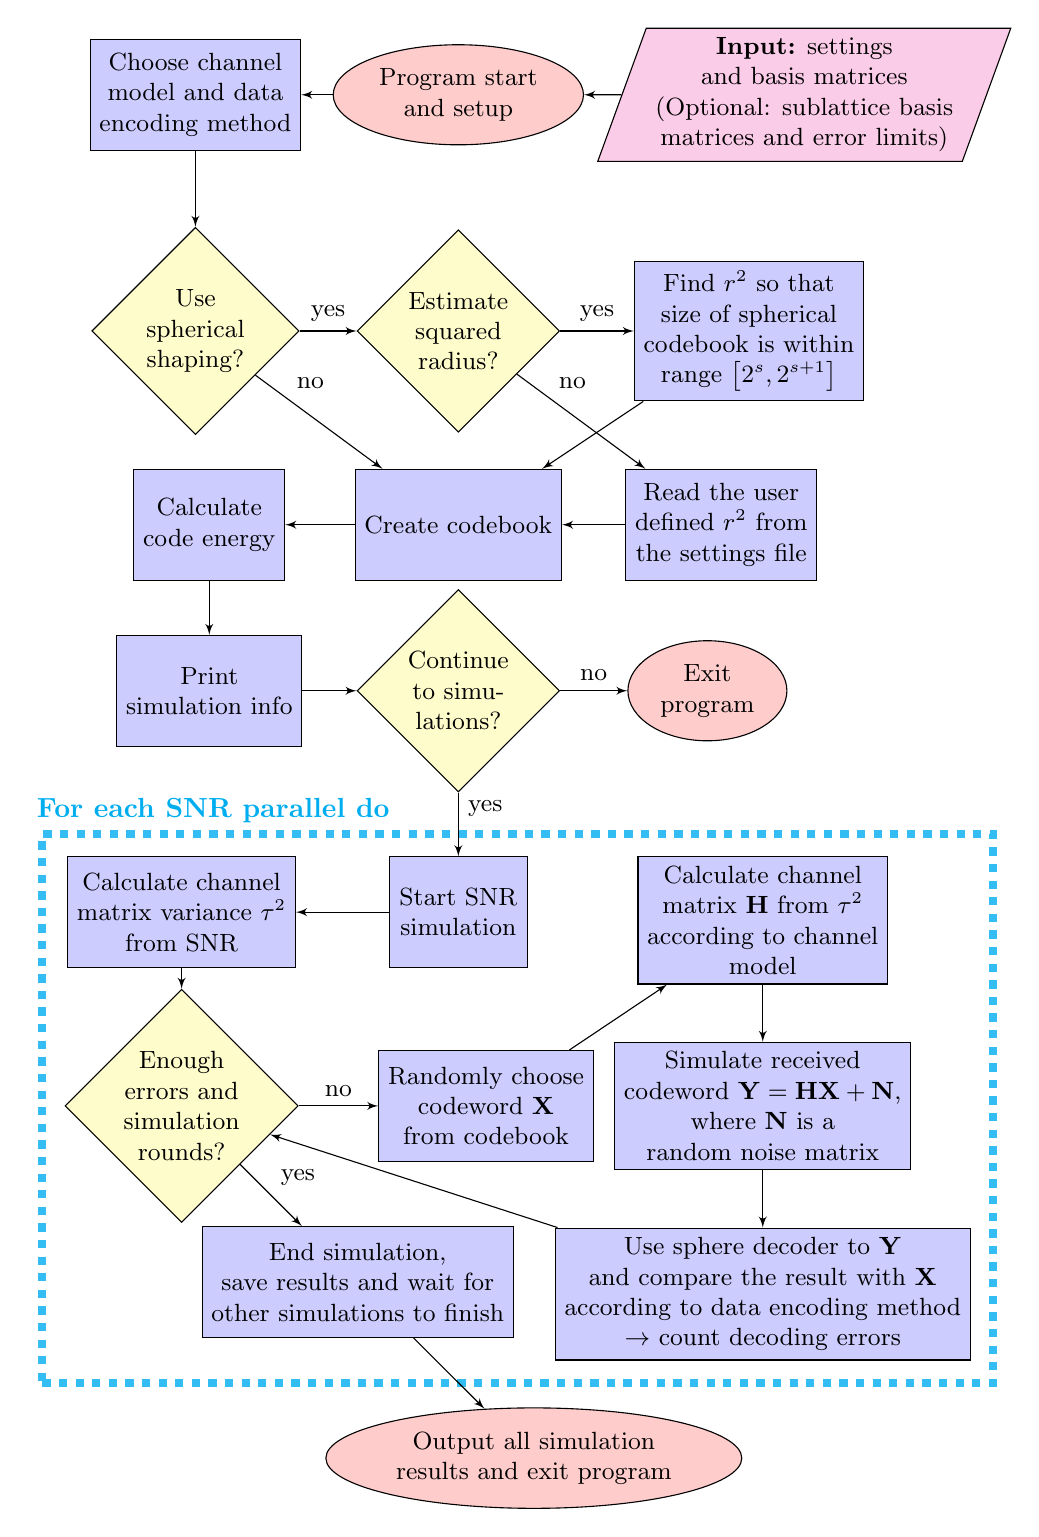
\begin{tikzpicture}[node distance = 5em, auto]
    % Place nodes
    \node [cloud, align=center] (main) {Program start\\ and setup};
    %\node [draw,trapezium,trapezium left angle=70,trapezium right angle=-70,minimum height=2em, fill=magenta!20, right of=main, node distance=12.5em,align=center] (input) {\textbf{Input:} settings\\ and basis matrices\\(Optional: sublattice basis\\ matrices and error limits)};
    \node [trapez, right of=main, node distance=12.5em, align=center] (input) {\textbf{Input:} settings\\ and basis matrices\\(Optional: sublattice basis\\ matrices and error limits)};
    \node [block, left of=main, align=center, node distance=9.5em] (choose) {Choose channel\\ model and data\\ encoding method};
    \node [decision, below of=main] (estimate) {Estimate squared radius?};
    \node [decision, left of=estimate, node distance=9.5em] (spherical) {Use spherical shaping?};
    \node [block, right of=estimate, node distance=10.5em,align=center] (radius) {Find $r^2$ so that\\ size of spherical\\ codebook is within\\ range $\left[2^s, 2^{s+1}\right]$};
    \node [block, below of=estimate, node distance=7em] (codebook) {Create codebook};
    \node [block, right of=codebook, node distance=9.5em,align=center] (readradius) {Read the user\\ defined $r^2$ from\\ the settings file};
    \node [block, left of=codebook, node distance=9em, align=center] (code-energy) {Calculate\\ code energy};
    \node [block, below of=code-energy,align=center, node distance=6em] (siminfo) {Print\\ simulation info};
    \node [decision, right of=siminfo, node distance=9em] (continue) {Continue to simulations?};
    \node [cloud, right of=continue, align=center, node distance=9em] (exit) {Exit\\ program};
    \node [block, below of=continue, node distance=8em, align=center] (startsim) {Start SNR\\ simulation};
    \node [block, left of=startsim, node distance=10em, align=center] (Hvar) {Calculate channel\\ matrix variance $\tau^2$\\ from SNR};
    \node [decision, below of=Hvar, node distance=7em] (loop) {Enough errors and simulation rounds?}; 
    \node [block, right of=loop, node distance=11em, align=center] (codeword) {Randomly choose\\ codeword $\mathbf{X}$\\ from codebook};
    \node [block, right of=codeword, node distance=10em, align=center] (simulate) {Simulate received\\ codeword $\mathbf{Y} = \mathbf{HX} + \mathbf{N}$,\\ where $\mathbf{N}$ is a\\ random noise matrix};
    \node [block, above of=simulate, node distance=6.7em, align=center] (channel) {Calculate channel\\ matrix $\mathbf{H}$ from $\tau^2$\\ according to channel\\ model};
    \node [block, below of=simulate, node distance=6.8em, align=center] (sphdec) {Use sphere decoder to $\mathbf{Y}$\\ and compare the result with $\mathbf{X}$ \\ according to data encoding method\\ $\rightarrow$ count decoding errors};
    \node [block, below right of=loop, node distance=9em, align=center] (end) {End simulation,\\ save results and wait for\\ other simulations to finish};
    \node [cloud, below right of=end, node distance=9em, align=center] (finish) {Output all simulation\\ results and exit program};
    
    % simulation frame
    \node [frame,fit=(startsim)(Hvar)(loop)(codeword)(channel)(simulate)(sphdec)(end)] (cyan) {};
	\node [anchor=north west, font=\color{cyan}\bf, xshift=-0.4em, yshift=1.5em] at (cyan.north west){For each SNR parallel do};
    
    % Draw edges
    \path [line] (input) -- (main);
    \path [line] (main) -- (choose);
    \path [line] (choose) -- (spherical);
    \path [line] (spherical) -- node {yes} (estimate);
    \path [line] (spherical) -- node [near start] {no} (codebook);
    \path [line] (estimate) -- node {yes} (radius);
    \path [line] (estimate) -- node [near start] {no} (readradius);
    \path [line] (radius) -- (codebook);
    \path [line] (readradius) -- (codebook);
    \path [line] (codebook) -- (code-energy);
    \path [line] (code-energy) -- (siminfo);
    \path [line] (siminfo) -- (continue);
    \path [line] (continue) -- node {no} (exit);
    \path [line] (continue) -- node [near start] {yes} (startsim);
    \path [line] (startsim) -- (Hvar);
    \path [line] (Hvar) -- (loop);
    \path [line] (loop) -- node {yes} (end);
    \path [line] (loop) -- node {no} (codeword);
    \path [line] (codeword) -- (channel);
    \path [line] (channel) -- (simulate);
    \path [line] (simulate) -- (sphdec);
    \path [line] (sphdec) -- (loop);
    \path [line] (end) -- (finish);

\end{tikzpicture}
\caption{The program flowchart.}
\label{fig:program}
\end{figure}

\subsection{Simulation examples}

 
\clearpage

\section{Summary}


\clearpage
%% The \phantomsection command is nessesary for hyperref to jump to the 
%% correct page, in other words it puts a hyper marker on the page.

\phantomsection
\addcontentsline{toc}{section}{\refname}
%\addcontentsline{toc}{section}{References}
\begin{thebibliography}{99}

\bibitem{mia} Mäki,\ M. \textit{Space-time block codes and the complexity of sphere decoding.} Doria, Referenced 10.7.2017. Available at
  \url{https://www.doria.fi/bitstream/handle/10024/54404/gradu2008maki-miia.pdf}
   
\bibitem{cassels} Cassels, J.W.S. \textit{An introduction to the Geometry of Numbers}, New York, Springer--Verlag, 1971.

\bibitem{agrell} Agrell, E., Eriksson, T. and Zeger, K. \textit{Closest point search in lattices} IEEE Transactions on Information Theory, Vol. 48, pp.2201-2214,
August 2002.

\bibitem{conway} Conway,\ J.H. and Sloane,\ N.J.A. \textit{Sphere packings, lattices and groups.} Third edition, New York, Springer--Verlag, 1998.

\bibitem{zamir} Zamir,\ R. \textit{Lattices are Everywhere.} EE - Systems, Referenced 15.8.2017. Available: \url{http://ita.ucsd.edu/workshop/09/files/paper/paper_312.pdf}

\bibitem{arma} Conrad Sanderson and Ryan Curtin.
\textit{Armadillo: a template-based C++ library for linear algebra.}
Journal of Open Source Software, Vol. 1, pp. 26, 2016.
\url{http://dx.doi.org/10.21105/joss.00026}

\bibitem{ranto} C. Hollanti and K. Ranto, \textit{Maximal orders in space-time coding: Construction and decoding}. International Symposium on Information Theory and Its Applications, Auckland, 2008, pp. 1-5. Available at \url{http://ieeexplore.ieee.org/stamp/stamp.jsp?arnumber=4895634}

\bibitem{damen} M.O. Damen,\ H. El Gamal,\ G. Caire \emph{On maximum-likelihood detection and the search for the closest lattice point} IEEE Transactions on Information Theory, Vol. 49, pp.2389-2402, October 2003. Available at \url{http://ieeexplore.ieee.org/document/1237128/}

%\bibitem{fplll} The FPLLL development team, \textit{fplll, a lattice reduction library.} 2016, Available at \url{https://github.com/fplll/fplll}


\end{thebibliography}

%% Appendices
%% Liitteet
\clearpage

\thesisappendix

\section{Program User Guide}

%\subsection{Abbreviations}
%\begin{tabular}{ll}
%SNR & Signal to noise ratio \\
%CPU & Central processing unit \\
%RAM & Random access memory \\
%GPU & Graphical processing unit \\
%C++ & C++ programming language \\
%OS & Operating system \\
%\end{tabular}

\subsection{Preface}
The purpose of this program is to simulate the performance of different space--time lattice codes under different levels of SNR. Its implementation heavily depends on C++ linear algebra template library called Armadillo \cite{arma}. This program is a console application (i.e. it is operated from command line) that uses simple text based files for input and output. It also has a optional plotting utility which provides graphical interface for the simulation results. The program is primalily intented to be used on Linux based operating systems but should be portable to other platforms as well (there are some slight differences in the required compiler instructions and used libraries though). If there are compatibility issues optional parts of the program can be left uncompiled intentionally. 
\par This guide assumes Linux based operating system, the steps described here might differ slightly when the program is used on other operating systems. The details regarding to those differences are not discussed here, but references to additional documentation are given. In the following chapters we will go through the installation and usage of the program in detail. 

\subsection{System requirements}
\label{sec:req}
%Regarding the hardware as the rule of the thumb, the better the performance your computer has the faster the simulations, although nearly all modern computers with a keyboard and a monitor should suffice for small simulations. The program makes use of parallel CPU cores so one does not need to worry too much about single thread performance of the CPU. The program should not be too memory consuming except in some special use cases so no excessive amount of RAM is needed for fast simulations. 
The program runs optimally on Linux and Mac OS and can make use of multiple CPU cores for parallel computing of the simulations. Windows is not recommended due to the limitations posed by the Armadillo library \cite{arma}. The hardware requirements for running small scale simulations are relatively low, any modern laptop should do.
\par One can optionally make use of the computing power of the GPU, which could potentially speed up large matrix operations that the linear algebra library Armadillo does. This requires CUDA toolkit and NVBLAS, see details here: \url{http://docs.nvidia.com/cuda/nvblas/index.html}. Keep in mind that this feature is somewhat experimental, so if you encounter any problems you can always recompile the program without this feature.
\par Before trying to install and run the program itself, you need to make sure you have GNU Make and a compatible C++ compiler installed. The recommended GNU C++ compiler (g++) and GNU Make should be preinstalled in most Linux distributions but in case they are not, try installing the \textit{build-essentials} package from the package manager. In Ubuntu you can do this by typing in terminal:
\begin{verbatim}
$ sudo apt-get install build-essential
\end{verbatim}
If this does not work please refer to \url{https://gcc.gnu.org/wiki/InstallingGCC} and \url{https://www.gnu.org/software/make/}. 
\par The next thing is to gather the required library packages:
\begin{enumerate}
\item OpenBLAS library: \url{https://github.com/xianyi/OpenBLAS/wiki/Installation-Guide}
\item LAPACK -- Linear Algebra PACKage: \url{http://www.netlib.org/lapack}
\item ARPACK library: \url{http://www.caam.rice.edu/software/ARPACK}
\item Armadillo C++ Linear algebra library: \url{http://arma.sourceforge.net/download.html} 
\item Boost C++ library (optional, for plotting only): \url{http://www.boost.org}
%\item MPFR 2.3.0 or higher (optional, for LLL reduction only) \url{http://www.mpfr.org/}
%\item GNU MP 4.2.0 or higher (optional, for LLL reduction only) \url{http://www.gmplib.org/}.
\end{enumerate}
% (libarmadillo-dev)
%Please note that the fplll library used for LLL reduction seems to only support reduction of integer matrices, which is not very reasonable assumption for communications applications like this, so \textbf{it is recommended for most users not to bother with the LLL reduction related functionality and simply leave it out (ie. not install packages 6 ja 7).} 
You can follow the links in the packege list for detailed instructions on how install those packages if you're facing problems (e.g. you're not installing the program on Linux) but the most straightforward way of installing them is by opening a terminal (in Linux CTRL+ALT+T) and using a package manager utility (e.g. apt-get in Ubuntu) to install those packages. The first three packages are required by the Armadillo library so you should install the packeges in the given order. Also note that not Linux based operating systems might require different libraries for Armadillo to work, in this case please refer to the Armadillo documentation by following the given link in the package list. 
\par In the Linux package manager the libraries listed should go by names: \textit{libopenblas-dev}, \textit{liblapack-dev}, \textit{libarpack-dev}, \textit{libarmadillo-dev}, \textit{libboost-all-dev}. %, \textit{libmpfr-dev} and \textit{libgmp-dev}. 
Note that there might be some version number before the first dash in those names. The Boost library can safely be omitted for compatibility reasons. If all the install processes succeed you are now all set up to install the program itself.

\subsection{Installing the program}

Open terminal (CTRL+ALT+T) and create a folder for the program 
\begin{verbatim}
$ mkdir sphere-decoder
$ cd sphere-decoder
\end{verbatim}Once you are in that folder copy the contents of this Gitlab repository there: \url{https://version.aalto.fi/gitlab/pasi.pyrro/sphere-decoder}. This requires you to have Aalto University login credentials. If you have trouble accessing the repository contact your supervisor who instructed you to use this program, they should have a copy of it. The copying from the repository can be done by either downloading the repository as a compressed folder (e.g. zip) and extracting it into the folder created earlier or by using the following command in the terminal (requires git to be installed on the system):
\begin{verbatim}
$ git clone git@version.aalto.fi:pasi.pyrro/sphere-decoder.git
\end{verbatim}

\noindent After copying the files check the contents of that folder by typing this command in the terminal:
\begin{verbatim}
$ ll
\end{verbatim}
Check if the contents of that folder look similar to those of the Gitlab repository. If everything looks all right, you're using Linux and want to do the plain installation (without plotting or GPU support), just type the following in terminal
\begin{verbatim}
$ make
\end{verbatim}
to compile the program. For other operating systems you likely need to modify the Makefile located in the /src/ directory. For convenience there is also a file called \textit{Makefile.mac} in /src/ directory. Replacing the default Makefile with that (by removing the file extension) should work for most MAC users. 
\par There are a couple of options how to compile the program if you did manage to install the required libraries. If you installed everything listed above and want to do the full installation, then type this instead.
\begin{verbatim}
$ make with=plotting+gpu
\end{verbatim}
You can choose also choose just one of those options, for example
\begin{verbatim}
$ make with=plotting
\end{verbatim} 
but keep in mind the requirements for them:
\begin{enumerate}
\item \textbf{plotting}: C++ Boost library
%\item \textbf{lll}: GMP, MPFR and you probably need to compile the fplll library \cite{fplll} in {/src/fplll} from source, see \url{https://github.com/fplll/fplll/#compilation} for help. Also remember to run the configure command like so
%\begin{verbatim}
%$ ./configure --prefix=$(pwd)/src/fplll/
%\end{verbatim} 
%so the library will be installed in the correct place. 
\item \textbf{gpu}: CUDA Toolkit and NVBLAS, see section \ref{sec:req}
\end{enumerate}
%If you didn't install the Boost C++ library you need to do the following in order to compile the program:
%\begin{verbatim}
%$ nano src/misc.hpp
%\end{verbatim}
%In the text editor locate a line of code saying
%\begin{verbatim}
%#define PLOTTING // enable plotting (requires boost C++ library)
%\end{verbatim}
%and either remove it or comment it out (type '//' in front of the line). After that save and exit by pressing CTRL+O, ENTER and CTRL+X. After that type the command:
%\begin{verbatim}
%$ nano src/Makefile
%\end{verbatim}
%and remove all the compiler flags that have the word 'lboost' in it. Save changes and exit the text editor as before. Now you should be able to compile the program by typing:
%\begin{verbatim}
%$ make
%\end{verbatim}

\noindent If the compiling succeeded, now check if the program runs correctly by typing:
\begin{verbatim}
$ make run
\end{verbatim}
%or by 
%\begin{verbatim}
%$ sh sphdec.sh
%\end{verbatim}
%if you're using the LLL reduction build.
If there are no errors regarding missing libraries or such then you have just correctly installed the program! If there are such errors during the compilation or program runtime, go back to previous section and double check that you have installed the correct libraries. 

\subsection{Setup and Input}

Now that the program is installed it is time to take a look at the simulation parameters and the program input files in order to run successful simulations. In the /bases/ folder there are text files containing the lattice code basis matrices for the simulation. These files are really important as they contain the lattice code itself, the performance of which you want to simulate. Note that the program supports complex matrices as input, which are the preferred way of inputting your basis matrices. You can (and should) add your own basis matrix text files there. The program should not be too picky about the input format but do make sure you have something other than white spaces separating the matrix entries. The most tested input format is the \href{http://reference.wolfram.com/language/tutorial/LinearAlgebraMatrixTypes.html#1527024338}{Wolfram Mathematica complex matrix format}, which should work in all cases. This format is also used in most of the example basis matrix files provided with the program, which you can use as a reference, like the one in figure \ref{fig:alamouti_basis}.
%The basis file for the Alamouti code should already be there and is used as the default. When creating a new basis file, one should stick to either Mathematica or Matlab syntax for complex matrices to ensure correct interpretation of the input. 
\begin{figure}[htb]
\begin{Verbatim}[frame=single]
{{1, 0},
{0, 1}}

{{0, -1},
{1, 0}}

{{0+I, 0},
{0, 0-I}}

{{0, 0+I},
{0+I, 0}}
\end{Verbatim}
\caption{An example basis matrix input file (alamouti.txt) for the Alamouti lattice code. It contains four 2x2 complex matrices, which form the base of the lattice code.}
\label{fig:alamouti_basis}
\end{figure}

\par For simulation parameters and other options one should navigate to /settings/ folder and open the default settings file called \textit{settings.ini}. The key contents of the file are displayed in figure \ref{fig:settings}. There are usually also comments in those settings files that start after the character sequence '//' and end in the line end but these are left out of the figures for clarity reasons. The comments are of course ignored by the program and only hold meaning for the user. Make sure not to remove any of the 22 options or the program will complain you about missing options. If you want to disable an option, it is done by either leaving the option value empty (string options) or setting it to -1 (number options) as seen in the figure \ref{fig:settings}. In case you end up messing up the settings file in some way, easy way to reset it is to just delete the file and run the program normally. This will generate a new default settings file for you, like the one in figure \ref{fig:settings}. 

%\begin{figure}[htb]
%\begin{center}
  %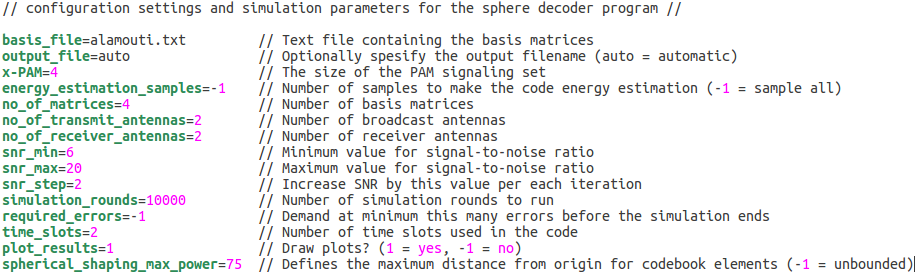
\includegraphics[width=\linewidth]{settings}
  %\caption{The default settings file for the sphere decoder program.}
  %\label{fig:settings}
%\end{center}
%\end{figure}

\begin{figure}[htb]
\begin{Verbatim}[frame=single, numbers=left]
basis_file=alamouti.txt
output_file=
coset_file=
error_file= 
channel_model=mimo            
x-PAM=4                         
energy_estimation_samples=-1   
no_of_matrices=4                
matrix_coefficient=1.0         
time_slots=2                    
no_of_transmit_antennas=2      
no_of_receiver_antennas=2    
snr_min=-6                      
snr_max=20                    
snr_step=2                    
simulation_rounds=10000       
required_errors=-1              
plot_results=-1    
stat_display_interval=-1        
spherical_shaping_max_power=-1
codebook_size_exponent=-1     
radius_search_density=100
\end{Verbatim}
\caption{The default settings file (settings.ini) for the sphere decoder program.}
\label{fig:settings}
\end{figure}

When editing the settings, only modify the right hand side of the equality sign. If you change the option variable names, the program will not recognise them. You can always check the correct variable names from figure \ref{fig:settings} or just generate a new default settings file if you happen to change them accidentally. 
%Another rule of the thumb is that if you want to use default behaviour for some feature, use -1 value for that variable. 
The order of the setting variables does not matter, just make sure they're all on their own separate line. Remember to save the changes you make to that file. The program doesn't need to be recompiled for these changes to take effect, just run it again after saving the settings file.
\par One can also create multiple settings files in that folder. To use a different settings file one just needs to give its name as a command line argument for the program. This will be explained in the next chapter. Using multiple settings files is really useful for organizing different simulations so you don't have to touch every parameter everytime you want to do a different simulation.

\subsection{Running the program}

Once the program is set up correctly, running the program is a relatively easy task. Just make sure you're in the root folder of the local repository (the folder where the program is located) and type the following in terminal:
\begin{verbatim}
$ make run
\end{verbatim}
or
\begin{verbatim}
$ ./sphdec [settings_file.ini*]
\end{verbatim}
%or 
%\begin{verbatim}
%$ sh sphdec.sh [settings_file.ini*]
%\end{verbatim}

\noindent The first command uses the default settings file and in the second one can optionally spesify the name of the settings file to be used (do not give the whole file path, just the name of a file in /settings/ folder). If no command line argument is given the first two commands are equal. %The last one is the same as the second one but it runs a shell script that sets an environment variable required to link the program with fplll library during runtime. Use this only if you compiled the program with LLL reduction support.
\par Once the program has started it prints useful data related to the current actions it is taking to the terminal as well as in the log.txt file located in the /logs/ folder. Visiting the log.txt file can be useful for reviewing previous program behaviour in the future. In the log file each program runtime should be separated by an empty line.
\par If the program gets stuck somewhere or takes too long to finish a large simulation, pressing CTRL+C in the terminal will terminate the execution of the program almost instantly. The program attempts to output the current simulation data even in this situation but it is not quaranteed to succeed so keep that in mind when doing that. For large simulations one needs to be patient as the simulation complexity grows exponentially with the lattice code dimension. It might be required to hit this key combination several times if the program does not terminate within five seconds or so.

\subsection{Output and Plots}

If the program exits without errors its output should be found from /output/ folder in csv format. This standard data format is easy to import into Matlab and other programs you might need. The filenames are by default named so that they are in chronological order so the latest simulation output should be the last one in the file listing. The csv format is easy to import in other programs like Matlab.
\par If the program was compiled successfully with the plotting make option and the following settings variable is set to
\begin{verbatim}
plot_results=1 
\end{verbatim}
then a couple of graphical interfaces for plots generated from the simulation data should pop up. If there are errors check that you also have GNUPlot installed on your system. Plotting gives you a quick review on how the simulation went. For more rigorous data analysis it is recommended to import the output csv file to some numerical scientific calculation software like Matlab.

\subsection{General troubleshooting}
Some general miscellaneous tips are listed here to help you troubleshoot errors while using the program:
\begin{enumerate}
\item Do not include the dollar sign in terminal commands. It's just there to indicate terminal input.
\end{enumerate}


\end{document}
